\documentclass[9pt,twocolumn,twoside]{../../styles/osajnl}
\usepackage{supertabular,booktabs}
\journal{i524} 

\title{Cloudmesh Docker Extension}

\author[1]{Karthick Venkatesan}
\author[2]{Ashok Vuppada}


\affil[1]{School of Informatics and Computing, Bloomington, IN 47408, U.S.A.}


\dates{S17-IR-P009, \today}

\ociscodes{Cloud, I524}

\doi{\url{https://github.com/cloudmesh/sp17-i524/blob/master/project/S17-IR-P009/report/report.pdf}}


\begin{abstract}
Cloudmesh client is a simple client to enable access to multiple cloud environments form a command shell and command line. The user's can manage their set of resources right from their workstation.Currently cloudmesh client supports managing Virtual Machines across multiple clouds. In this project we have added the capability to manage/provision docker and swarm containers to cloudmesh client through a simple and extensible command line interface.

\end{abstract}

\setboolean{displaycopyright}{true}

\begin{document}


\maketitle


\section{Introduction}
In the time of Big data and Micro-Services,it is common to have a set of services running on multiple clouds.Docker\cite{www-Docker} with the build and ship model made the micro-services architecture work better.Since there would multiple containers running across multiple remote clouds managing them can become tedious.In project we have added the capability to provision and manage docker\cite{www-Docker} and swarm\cite{www-Swarm} containers to cloudmesh client\cite{las14cloudmeshmultiple}.

Clouldmesh Client\cite{las14cloudmeshmultiple} capability is detailed in Figure~\ref{fig:cmvm},it aims at managing vm instances in multiple heterogeneous clouds remotely via a command line interface.

\begin{figure}[h!]
\centering
\fbox{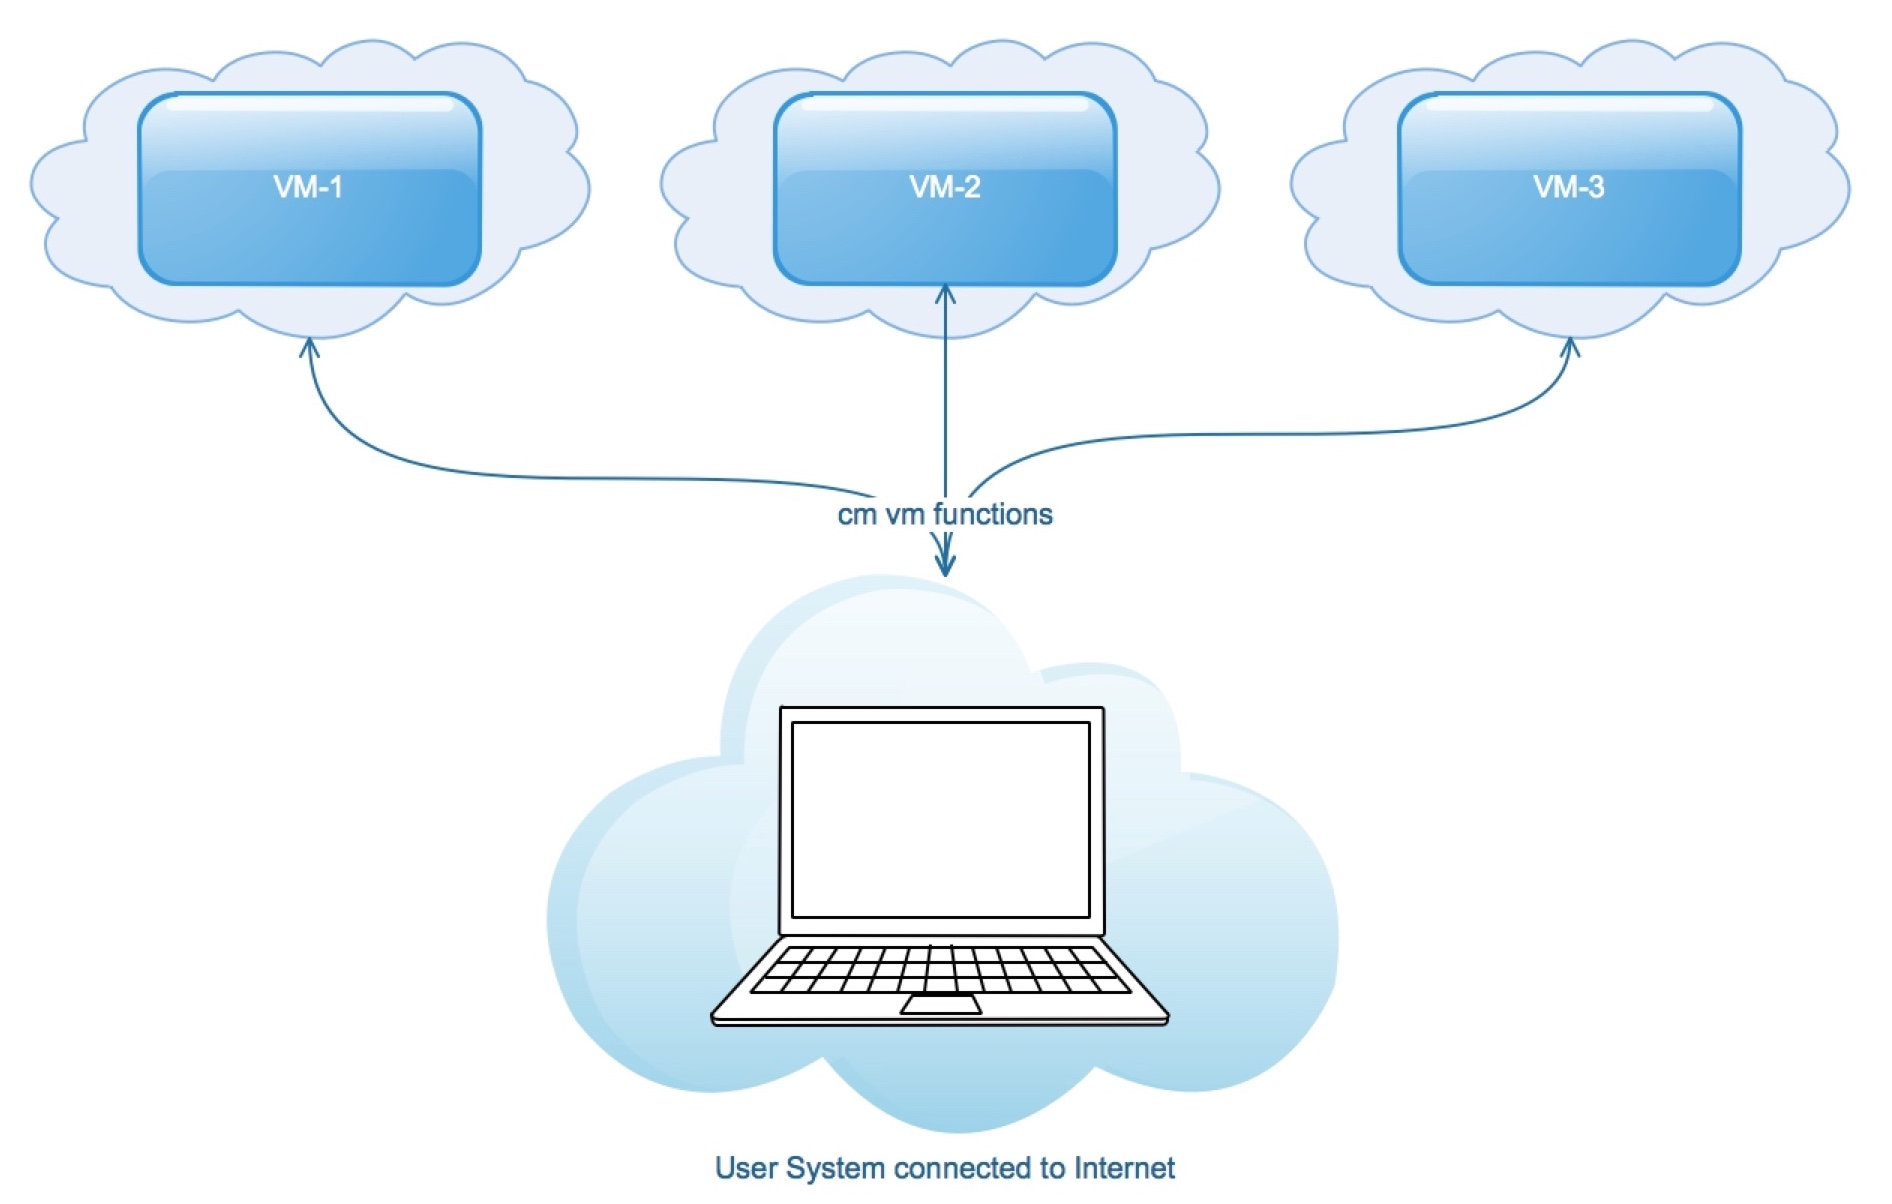
\includegraphics[width=\linewidth]{images/cmvm.jpeg}}
\caption{Cloudmesh client }
\label{fig:cmvm}
\end{figure}

The cloudmesh docker application build  can be broadly divided into Docker and Swarm modules.\\

The Docker Module capabilities are detailed in
Figure~\ref{fig:cmsdocker}. This module would help user perform
various docker functions mentioned in Section 3 

\begin{figure}[h!]
\centering
\fbox{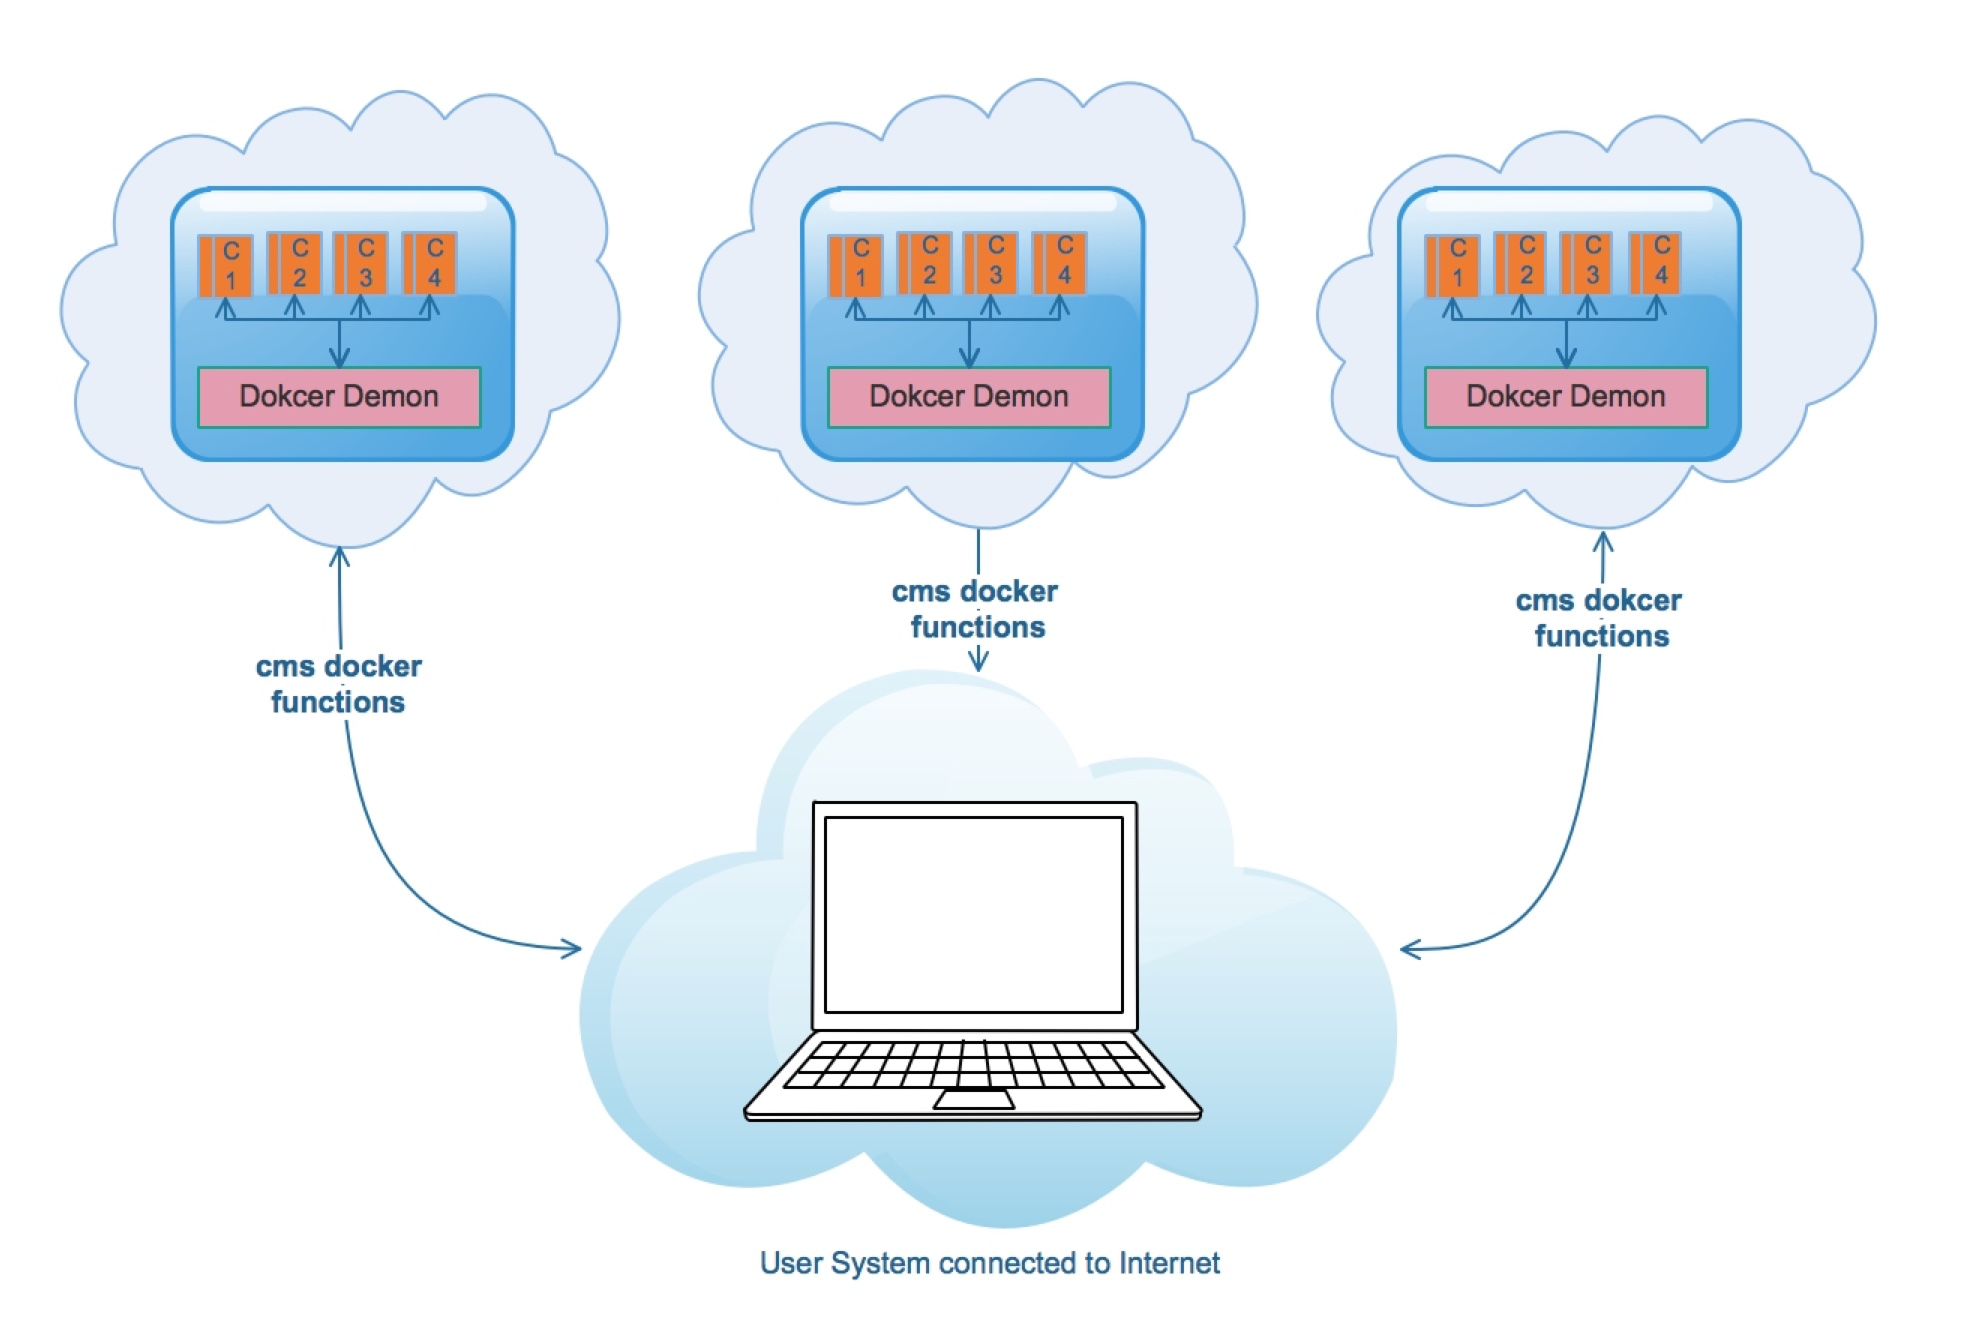
\includegraphics[width=\linewidth]{images/cmsdocker.jpeg}}
\caption{Docker Mode }
\label{fig:cmsdocker}
\end{figure}

The Swarm module facilitates performing various swarm operations Figure~\ref{fig:cmsswarm}.

\begin{figure}[h!]
\centering
\fbox{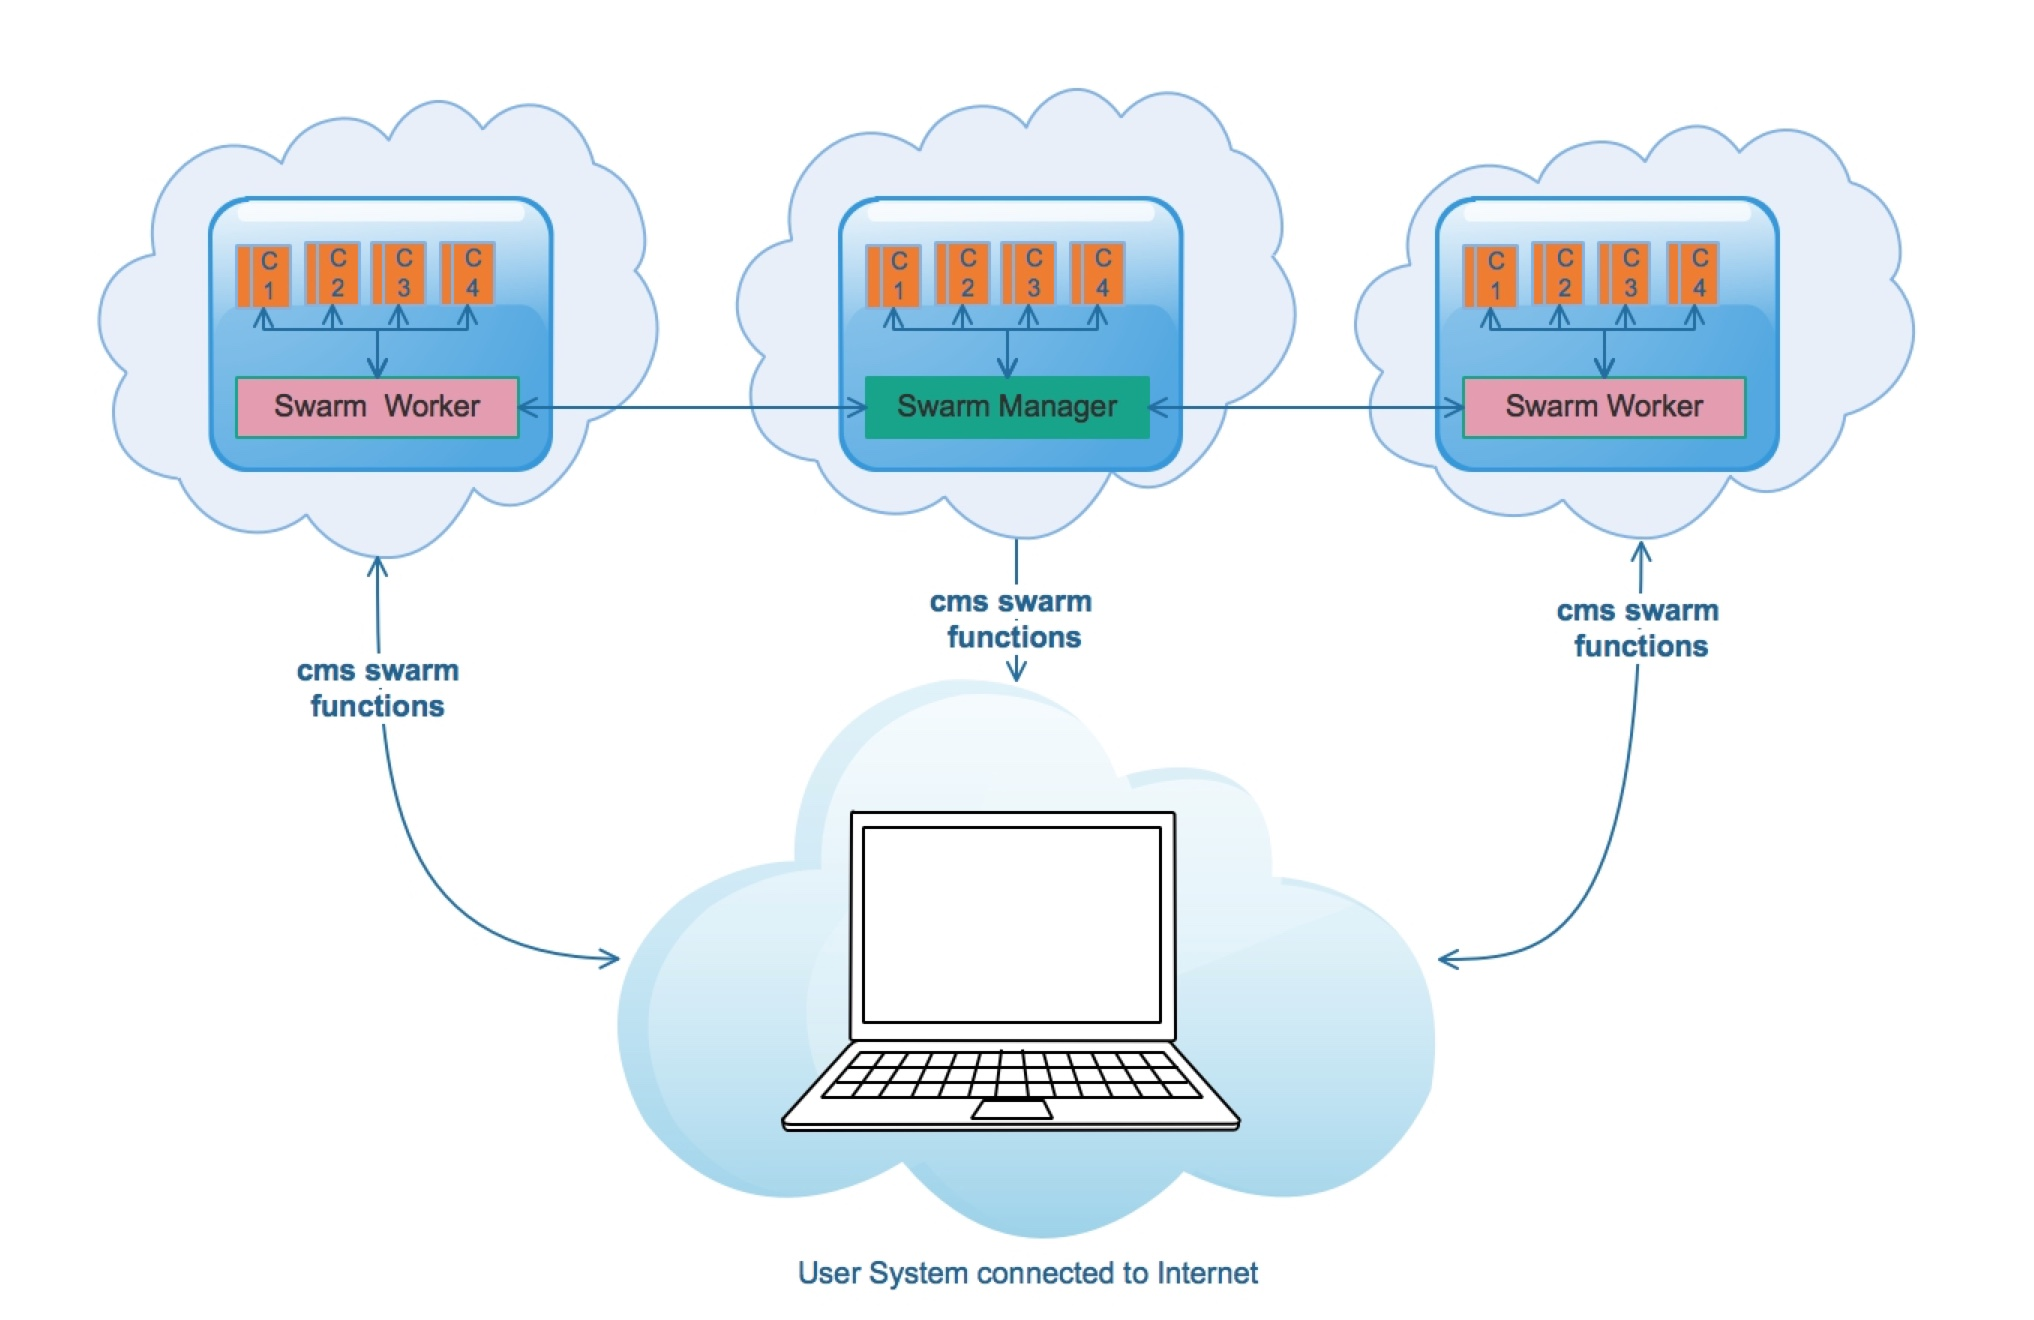
\includegraphics[width=\linewidth]{images/cmsswarm.jpeg}}
\caption{Swarm Mode }
\label{fig:cmsswarm}
\end{figure}

Users can choose to use cloudmesh docker application from a remote terminal outside the network of the data center as in ~Figure\ref{fig:cmsdocker} or locally from a provisioning or configuration server inside the data center as in Figure~\ref{fig:cmsdocker-2}
\begin{figure}[h!]
\centering
\fbox{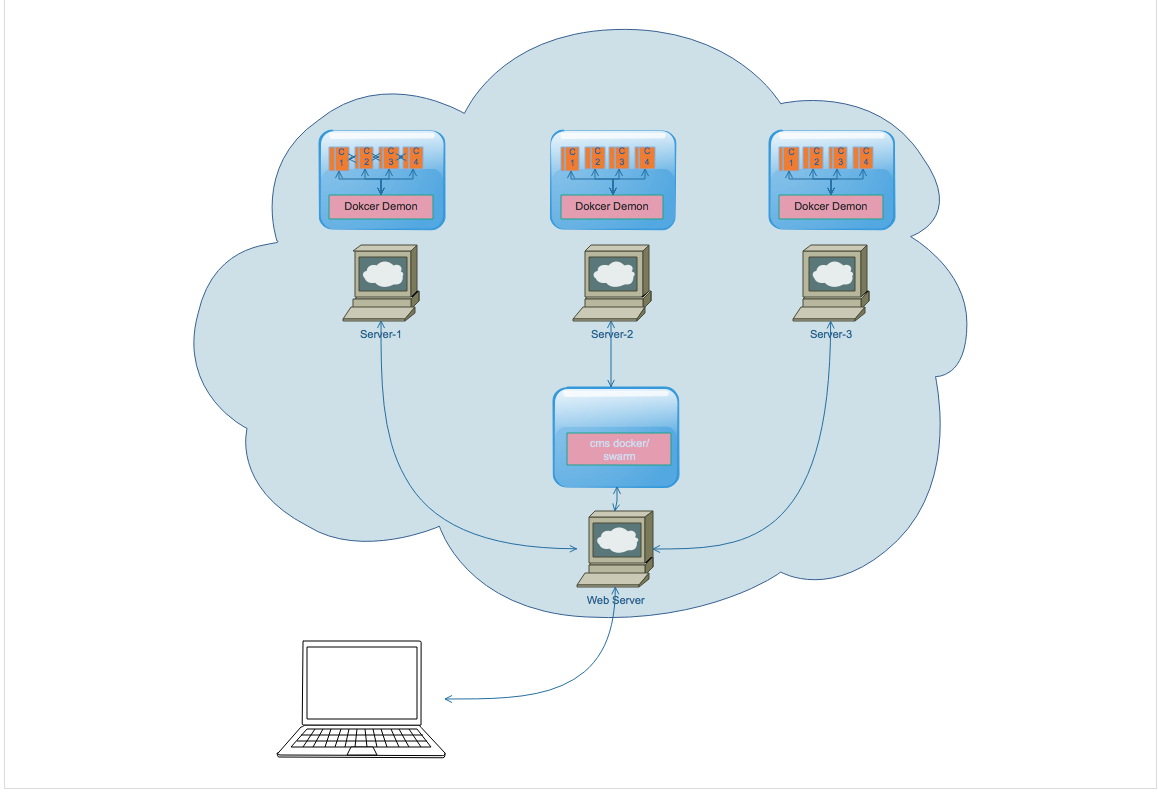
\includegraphics[width=\linewidth]{images/cmsdocker-2.png}}
\caption{Docker/Swarm Remote }
\label{fig:cmsdocker-2}
\end{figure}



\section{Application Architecture}
The architecture of the application is depicted in Figure~\ref{fig:Arch}.The commands developed can be broadly classified as 'action commands','Inquiry commands'.\\
The action commands are which would create or alter an entity.The entity can be a host/container/node. we use the corresponding API call to get the latest values for the changed entity.Docker API module is developed for addressing the docker commands and Swarm API module is used for swarm commands.\\
The Inquiry commands have two flavours a list and refresh mode.The list commands fetch the data locally from the Database and the refresh command will refresh the current state of the corresponding entity from the hosts.

\subsection{Technologies Used}
\begin{table}[H]
\centering
\begin{tabular}{|c c|} 
 \hline
 Name & Purpose \\ 
 \hline
 docker \cite{www-Docker} & Docker Server and Api for managing containers \\ 
 mongodb \cite{www-MongoDB} & Nosql DBMS \\ 
 Python-eve    \cite{www-Pythoneve} & Restful webservices interface to mongoDB \\ 
 python \cite{www-Python} & development  \\ 
 ansible \cite{www-Ansible} & automated deployment \\ [1ex] 
\hline
\end{tabular}
\caption{Technology Name and Purpose}
\label{table:1}
\end{table}

\subsection{MongoDB and Python-eve}

The cloudmesh docker application uses MongoDB\cite{www-MongoDB} for data storage.The access to the database is all through
restful services supported through Python-eve\cite{www-Pythoneve}.The following are the entities for which collections are defined 
in eve and mongoDB.

\begin{enumerate}
\item Host
\item Image
\item Container
\item Network
\item Service
\item Node
\end{enumerate}
A key benefit of using a NoSQL data base like mongoDB is that it allowed us to store the data in the the DB in the native form as returned by the Docker Api without the need for much marshaling of the data .The application uses the cloudmesh.rest repository for managing mongo and eve services.


\begin{figure}[htbp]
\centering
\fbox{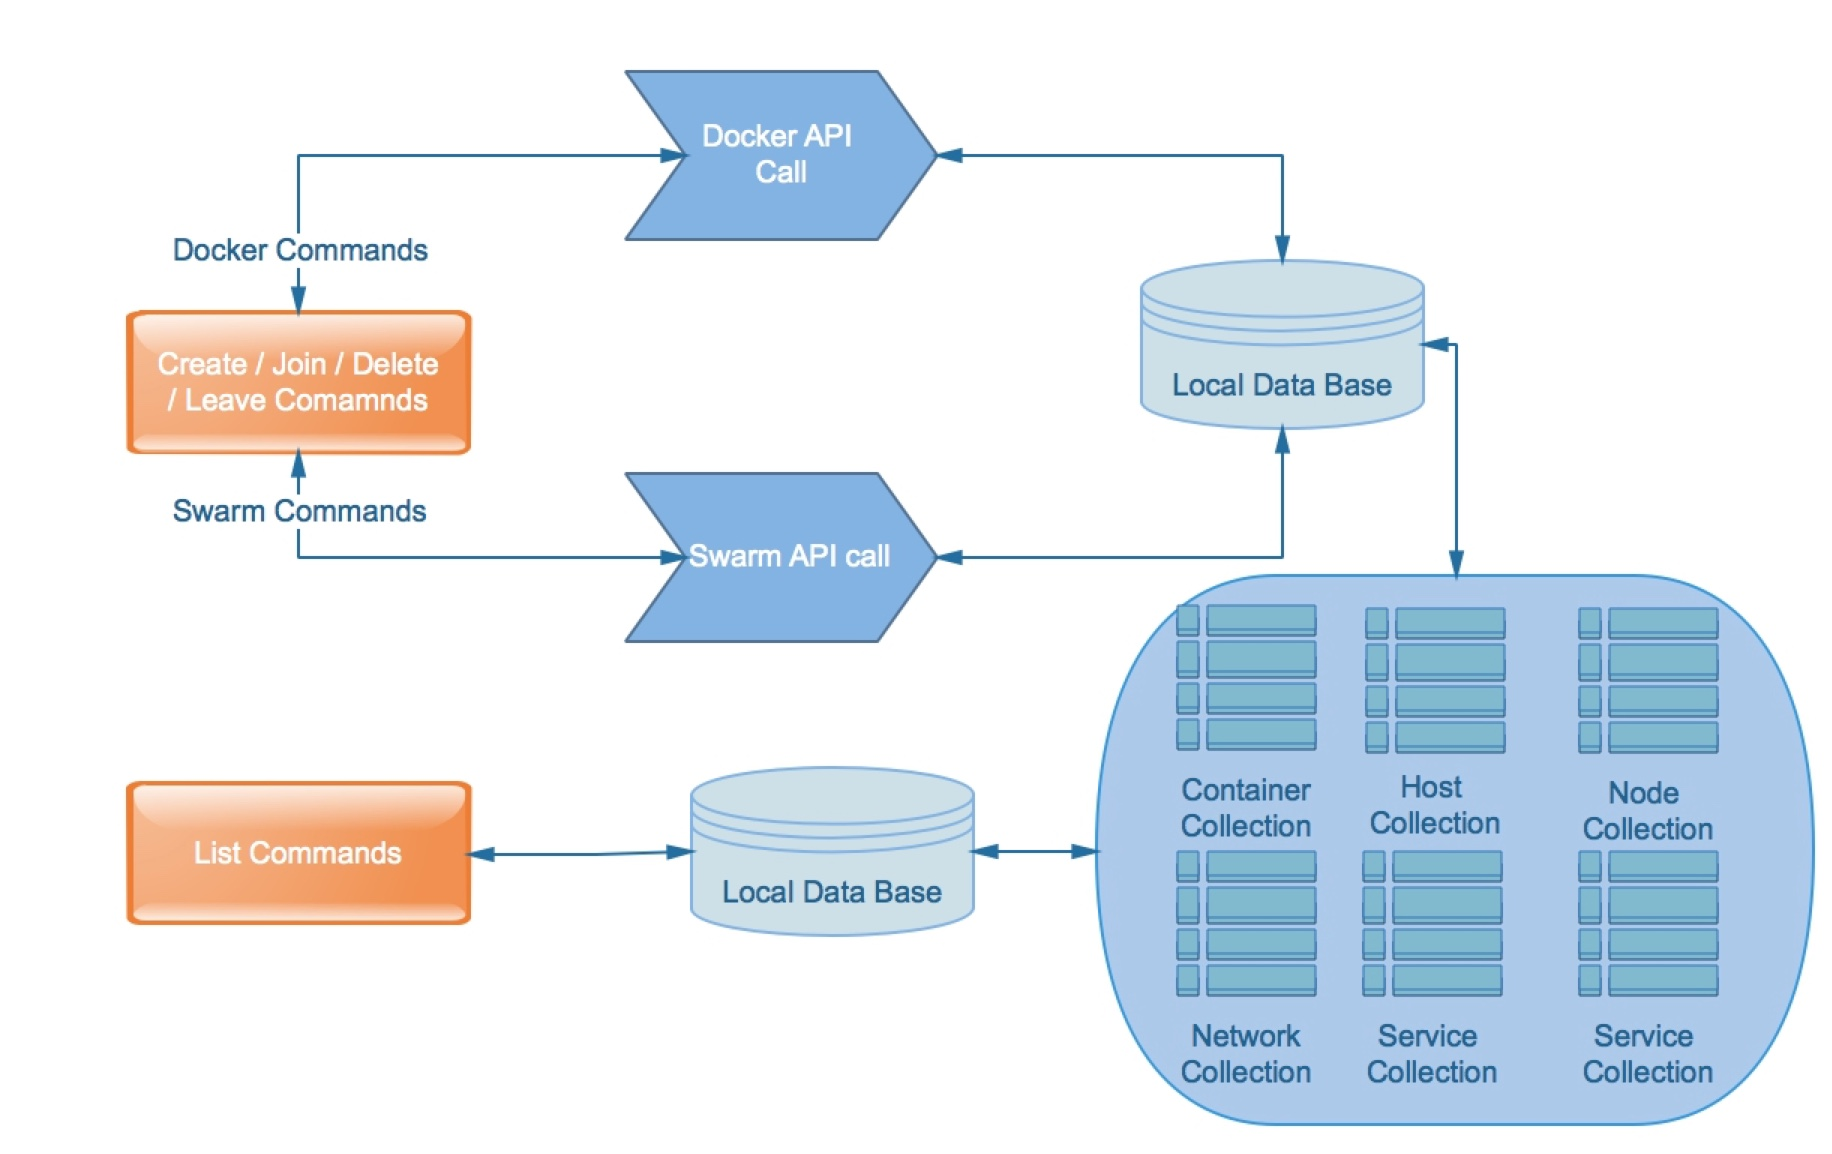
\includegraphics[width=\linewidth]{images/Arch.jpeg}}
\caption{cms docker extension application architecture}
\label{fig:Arch}
\end{figure}

\subsection{Cloudmesh Common}

The application makes extensive use of common functions and tightly integrated into common functions available in the cloudmesh common repository for display formatting , YAML config management and timers

\subsection{Ansible}

As part of the project we have built Ansible\cite{www-Ansible} scripts to automate installation of docker in remote hosts and also deployment of docker images in these remote docker hosts.Below is the list of Ansible scripts that are built and used in the project 
\begin{enumerate}
\item Install Docker in remote hosts and enable them for remote API access
\item Install Docker images in docker hosts .As part of the script the local docker files are synced with remote hosts and the images are built .
\item Setup /etc/hosts for remote hosts.This script allows to setup host names and IP in remote hosts which allows the applications to be configured to access by the standard host names instead of the IP address of the machine.
\end{enumerate}

\section{Docker Commands}
\begin{enumerate}
    \item\textbf{Host Set/Add}
     This command is to be used to setup the docker host on which the user wants to operate .The docker commands following would be executed on the host setup in this step. The host details will be also captured in the database with this command.
    \begin{verbatim} cms docker host docker1 docker1:4243 \end{verbatim}
    
    \item \textbf{Host List}
     This command would list the hosts available.This command would display the Ip,Name,Port,and if the host is swarm manager and the swarm manager Ip. Please note the Swarmmanager Ip would be blank if the host is manager or not part of swarm. 
     \begin{verbatim}
     cms docker host list 
     \end{verbatim}
     
     \begin{table}[h!]
     \caption{\bf cms docker host list }
     \begin{tabular}{ccccc}
     \hline
      Ip & Name & port & Swarmmode &SwarmManagerIp\\
      \hline
      docker1 & docker1 & 4243 & Manager & \\
      docker2 & docker2 & 4243 & Worker & docker1\\
      docker3 & docker1 & 4243 & Host & \\
     \hline
     \end{tabular}
     \label{tab:tab1}
     \end{table}
     
    \item \textbf{Host Delete}
    This command would be used to delete a host from the setup.This would also delete the host details from the database.User can do a host list to see the updated host details.\\
    \begin{verbatim}
    cms docker host delete docker1:4243
    \end{verbatim}
    
    \item \textbf{Image List}
    This command would be used to display the images available on a host.
    It would display the Ip of the host,the Image id , repository and the size of the image.Please note that this command would display the results from the local dB.\\
    \begin{verbatim}
    cms docker image list
    \end{verbatim}
    
    \begin{table}[h!]
     \caption{\bf cms docker image list }
     \begin{tabular}{cccc}
     \hline
      Ip & Id & Repository & Size(GB)\\
      \hline
      docker1 & 5545f4e3b27e & cloudmesh:docker & 5.59 \\
      docker2 & 45f4e3b2799e & elasticsearch:swarm & 0.45 \\
     \hline
     \end{tabular}
     \label{tab:tab2}
     \end{table}
     
    \item \textbf{Image Refresh} 
     This command would refresh the images across the hosts available the results would update the local data base , and display the updated reults to the user.
    \begin{verbatim}
    cms docker image refresh
    \end{verbatim}

    \item \textbf{Container Create}
     This command would used to create a container on a given host.The arguments for this command would be the name of the container and the image from which the container needs to be created.The image in the argument must be available through image list command above on the given host.\\
 
    \begin{verbatim}
    cms docker container create test1 \
    elasticsearch:docker
    \end{verbatim}
    
    \item \textbf{Container Start}
     This command would be used to start a container.The container should be already created using the above command.\\

    \begin{verbatim}
    cms docker container start test1
    \end{verbatim}     
     
    \item \textbf{Container Stop}
     This command would be used to stop and container which is running.The container can be started using the above command\\

    \begin{verbatim}
    cms docker container stop test1
    \end{verbatim}  
    
    \item \textbf{Container List}
     This command would display the list of containers running across the hosts.This would return the Ip,Container Id , Name , Image , status and start time of the container.The details would be shown from the local database maintained.
     
    \begin{verbatim}
    cms docker container list
    \end{verbatim}  
        
     \begin{table}[h!]
     \caption{\bf cms docker container list }
     \begin{tabular}{cccccc}
     \hline
      Ip & Id & Name & Image &Status&StartedAt\\
      \hline
      docker1 & 5545f4e3b27e & test1 & image1 &exited & 12.00PM \\
     \hline
     \end{tabular}
     \label{tab:tab3}
     \end{table}
     
    \item \textbf{Container Refresh}
     This command would refresh the current state of the containers across the hosts, This command would connect to the host and run the native docker container list to get the latest information and update the local database for refreshing the data. \\
     
    \begin{verbatim}
    cms docker container refresh
    \end{verbatim}  
    
    \item \textbf{Container Delete}
     This command would be used to delete a required container on the host. The arguments required are the container name.The updated container list can be viewed by running cms docker container list command.\\
     
    \begin{verbatim}
    cms docker container delete test1 
    \end{verbatim}  
    
    
    \item \textbf{Container Run}
     This command would be used to run a container instead of creating and starting in two steps.This arguments for the function are the name of the container and the image from which it needs to be run.\\
     
    \begin{verbatim}
    cms docker container run test1 /
    elasticsearch:docker
    \end{verbatim}  

    \item \textbf{Container Pause}
     This command would pause the container which is currently running.Use can run a cms docker container list to observe the status change.\\
     
    \begin{verbatim}
    cms docker container pause test1
    \end{verbatim} 

    \item \textbf{Container Unpause}
     This command would unpause the container which is currently paused.Use can run a cms docker container list to observe the status change.\\
     
    \begin{verbatim}
    cms docker container unpause test1
    \end{verbatim} 

    \item \textbf{Network Refresh}
    This command would refresh the network across the docker containers and hosts the updated results would be stored in the local database.
    
    \begin{verbatim}
    cms docker network refresh
    \end{verbatim} 

    \item \textbf{Network List}
    This command would display the results of the refreshed network.This would display the host ip where the network established , the network id , name and containers in the network\\

    \begin{verbatim}
    cms docker network list
    \end{verbatim} 
    
    \begin{table}[htbp]
     \caption{\bf cms docker network list }
     \begin{tabular}{cccc}
     \hline
      Ip & Id & Name & Containers\\
      \hline
      docker1 & 5545f4e3b27e & network1 & test1  \\
     \hline
     \end{tabular}
     \label{tab:tab4}
     \end{table}
\end{enumerate}


\section{Swarm Commands}
\begin{enumerate}
    \item \textbf{Host Set/Add}
     The command would be used to setup the current host.The docker commands following would be executed on the host setup in this step. the host details will be also captured in the database with this command.\\
     
    \begin{verbatim}
    cms swarm host docker1 docker1:4243
    \end{verbatim} 

     
    \item \textbf{Host List}
     This command would list the hosts available,This command would display the Ip,Name,Port,and if the host is swarm manager and the swarm manager Ip. Please note the Swarmmanager Ip would be blank if the host is manager or not part of swarm.
     
    \begin{verbatim}
    cms swarm host list
    \end{verbatim} 

     \begin{table}[htbp]
     \caption{\bf cms docker host list }
     \begin{tabular}{ccccc}
     \hline
      Ip & Name & port & Swarmmode &SwarmManagerIp\\
      \hline
      docker1 & docker1 & 4243 & Manager & \\
      docker2 & docker2 & 4243 & Worker & docker1\\
      docker3 & docker1 & 4243 & Host & \\
     \hline
     \end{tabular}
     \label{tab:tab5}
     \end{table}
     
    \item \textbf{Host Delete}
    This command would be used to delete a host from the setup.This would also delete the host details from the database.User can do a host list to see the updated host details.\\

    \begin{verbatim}
    cms swarm host delete docker1:4243
    \end{verbatim} 
    
    \item \textbf{Image List}
    This command would be used to display the images available on a host.
    It would display the Ip of the host,the Image id , repository and the size of the image.Please note that this command would display the results from the local dB.\\
    
    \begin{verbatim}
    cms swarm Image list
    \end{verbatim} 

    
    \item \textbf{Swarm Create}
    This would create swarm on the host in use.There is no arguments required for this command, After this command is run the current host status would be treated as 'manager'.user can run a node list or host list to see the updated result.To setup the current host user needs to use cms swarm host ADDR command shown above.\\
    
    \begin{verbatim}
    cms swarm create
    \end{verbatim} 
    
    \item \textbf{Swarm Join}
    This command would be applicable for the host which is not manager,user needs to setup a new current host with cms swarm host command and run cms swarm join so that current host would be joined with the swarm created in the last step.User needs to pass the swarm host Ip and address the host being joined\\
    
    \begin{verbatim}
    cms swarm join docker3 docker4:4243 worker
    \end{verbatim} 
    ( assuming docker3 is already a swarm manager) 
    
    \item \textbf{Swarm Leave}
    This command is applicable for the swarm manager or worker , this would let the host leave swarm.If manager has multiple workers ,workers needs to be removed(leave) before manager can leave.This command would treat current host is to be removed(leave) the swarm.User may need to set up the current host before processing the command.\\
    
    \begin{verbatim}
    cms swarm leave 
    \end{verbatim}

    
    \item \textbf{Network Create}
    This command would be used to create the network which can be used by the swarm containers later.The arguments it would need is the name of the containers.
    
    \begin{verbatim}
    cms swarm network create network1 
    \end{verbatim}
    
    \item \textbf{Network List}
     This command would display the results of the refreshed network.This would display the host ip where the network established , the network id , name and containers in the network\\
     
    \begin{verbatim}
    cms swarm network list  
    \end{verbatim}
    
    \begin{table}[htbp]
     \caption{\bf cms swarm network list }
     \begin{tabular}{cccc}
     \hline
      Ip & Id & Name & Containers\\
      \hline
      docker1 & 5545f4e3b27e & network1 & test1  \\
     \hline
     \end{tabular}
     \label{tab:tab6}
     \end{table}
     
    \item \textbf{Network Refresh}
    This command would refresh the network across the docker containers and hosts the updated results would be stored in the local database.\\
    
    \begin{verbatim}
    cms swarm network refresh  
    \end{verbatim}
    
    
    \item \textbf{Network Delete}
    This command would be used to delete an existing network.The inputs required for this command is just the network name.
    
    \begin{verbatim}
    cms swarm network delete network1  
    \end{verbatim}
    
    
    \item \textbf{Service Create}
    This command would be used to create a service,the arguments required are the image name and the name of service.This command would record the service details into the local database.\\
    
    \begin{verbatim}
    cms swarm service create elasticsearch \
    elasticsearch:swarm  
    \end{verbatim}
    
    \item \textbf{Service List}
    This command would list the current services running ,the data being displayed would be from the local data base, if the most current details are required user can run service refresh command below.\\

    \begin{verbatim}
    cms swarm service list 
    \end{verbatim}  
    
    The number of replicas below indicates the number of containers which are running the services.\\
    \begin{table}[htbp]
     \caption{\bf cms swarm service list }
     \begin{tabular}{ccccc}
     \hline
      Ip & Id & Name &Image & Replicas\\
      \hline
      docker1 & 5545f4e3b27e & elasticsearch &elastic:swarm  & 3  \\
     \hline
     \end{tabular}
     \label{tab:tab7}
     \end{table}
     
    \item \textbf{Service Delete}
    This command would be used to delete a running service,the arguments required are the service name.This command would delete the service details into the local database.\\
    
    \begin{verbatim}
    cms swarm service delete elasticsearch
    \end{verbatim} 
    
    \item \textbf{Service Refresh}
    This command would be used to refresh the services status based on the current condition.This command would refresh the local database so that service list would show the updated results.
 
    \begin{verbatim}
    cms swarm service refresh
    \end{verbatim} 
       
    \item \textbf{Node List}
    This command would display the list of the nodes across the hosts available.The results would come from the local database. The command would display the node id,,Id,Role,status and Manager Ip.
    
    \begin{verbatim}
    cms swarm node list
    \end{verbatim} 

     \begin{table}[htbp]
     \caption{\bf cms swarm node list }
     \begin{tabular}{ccccc}
     \hline
      Id & Ip & Role &Status & Manager Ip\\
      \hline
      5545f4e3b27e &docker3& Manager&Ready&  \\
      7645f4f4b27e &docker2& Worker&Ready&docker4  \\
     \hline
     \end{tabular}
     \label{tab:tab8}
     \end{table}
     
    \item \textbf{Image Refresh}
    This command would refresh the images across the hosts available the results would update the local data base , user can run docker image list to view the updated results.
    
    \begin{verbatim}
    cms swarm image refresh
    \end{verbatim} 
     
    \item \textbf{Image List}
    This command would be used to display the images available on a host.
    It would display the Ip of the host,the Image id , repository and the size of the image.Please note that this command would display the results from the local dB.\\
    
    \begin{verbatim}
    cms swarm image list
    \end{verbatim} 
    
    \begin{table}[htbp]
     \caption{\bf cms swarm image list }
     \begin{tabular}{cccc}
     \hline
      Ip & Id & Repository & Size(GB)\\
      \hline
      docker1 & 5545f4e3b27e & cloudmesh:docker & 5.59 \\
      docker2 & 45f4e3b2799e & elasticsearch:swarm & 0.45 \\
     \hline
     \end{tabular}
     \label{tab:tab9}
     \end{table}
     
    \item \textbf{Container Refresh}
    This command would refresh the current state of the containers across the hosts, This command would connect to the host and run the native docker container list to get the latest information and update the local database for refreshing the data. \\
    
    \begin{verbatim}
    cms swarm container refresh
    \end{verbatim} 

    \item \textbf{Container List}
    This command would display the list of containers running across the hosts.This would return the Ip,Container Id , Name , Image , status and start time of the container.The details would be shown from the local database maintained.
    
    \begin{verbatim}
    cms swarm container list
    \end{verbatim} 
    
     \begin{table}[htbp]
     \caption{\bf container list }
     \begin{tabular}{cccccc}
     \hline
      Ip & Id & Name & Image &Status&StartedAt\\
      \hline
      docker1 & 5545f4e3b27e & test1 & image1 &exited & 12.00PM \\
     \hline
     \end{tabular}
     \label{tab:tab10}
     \end{table}
\end{enumerate}

\section{Use Case - Elasticsearch cluster }
 Elasticsearch\cite{www-ElasticSearch} is an open-source, broadly-distributable, readily-scalable, enterprise-grade search engine. Accessible through an extensive and elaborate API, Elasticsearch can power extremely fast searches that support your data discovery applications[2]

 Using Cloudmesh  client , Ansible and Cloudmesh Docker application we deployed  and provisioned a Elasticsearch cluster on remote  hosts in Chameleon cloud in docker and swarm mode .We benchmarked the cluster using esrally\cite{www-ElasticSearchRally}  have compared  the  results between the elastic search clusters in docker and swarm mode.
 
 
 \subsection{Elasticsearch Cluster Docker Mode}
  For provisioning the Elasticsearch cluster in docker hosts below are the steps done
\begin{enumerate}
\item Created 3 Virtual Machines using Cloud Mesh Client .2 of the Virtual Machines  are to be used for the docker Elasticsearch cluster and 1 Virtual machine is the Benchmark server for the Kibana and esrally docker images 
\item Using Ansible scripts Install docker in 3 Virtual Machines and enable the docker daemon for remote access.
\item Using Ansible scripts Install Images of Elasticsearch  on hosts for docker cluster and the Image of Esrally in the Benchmark server .
\item Using the Cloudmesh Docker application we start 4 containers 2 in each of the virtual machines .To enable clustering of Elasticsearch applications running in the docker containers we need set the below parameters in container creation
\begin{verbatim}
    network_mode=host 
    environment=
    ["http.host=0.0.0.0",
    "transport.host=0.0.0.0",
    "discovery.zen.ping.unicast.hosts=docker1,docker2"]
\end{verbatim}

The network mode set to host allows the Elasticsearch containers use the underlying Virtual Machines  network for networking and leveraging the Elasticsearch unicast discovery find and form a cluster along with the other Elasticsearch instances running in other
containers either on the same host or different hosts.

\end{enumerate}

 \subsection{Elasticsearch Cluster Swarm Mode}
  For provisioning the Elasticsearch cluster in docker hosts in swarm mode below are the steps done
\begin{enumerate}
\item Created 3 Virtual Machines using Cloud Mesh Client .2 of the Virtual Machines  are to be used for the docker Elasticsearch cluster and 1 Virtual machine is the Benchmark server for the Kibana and esrally docker images 
\item Using Ansible scripts Install docker in 3 Virtual Machines and enable the docker daemon for remote access.
\item Using Ansible scripts Install Images of Elasticsearch  on hosts for docker cluster and the Images of Kibana and Esrally in the Benchmark server .
\item Using the Cloudmesh Docker application we first create a swarm cluster with the two docker hosts.Then we create a service in the Swarm  Manager Node.Along with the creation of the service we pass parameters to specify the number of replicas ,the network to be used , the mode of replication and the service name.
\begin{verbatim}
    ServiceMode.mode="replicated" 
    ServiceMode.replicas=4 
    EndpointSpec.ports=["9200:9200"] 
    networks=["elastic_cluster"] 
    env=["SERVICE_NAME=elasticsearch"]
\end{verbatim}

Swarm mode containers cannot use the the underlying host network as in the docker mode to enable the communication between the swarm containers we created a "overlay" network in the swarm manager.This network is passed in the service creation.So every container that is created by the swarm mode Manager will run on  this network .In the swarm mode to enable elastic search unicast discovery on start of the elastic search cluster using the Servicename environmental variable we identify other containers available in the cluster and dynamical set the \begin{verbatim} discovery.zen.ping.unicast.hosts \end{verbatim} parameter to enable elastic search to find and form a cluster with other Elasticsearch applications in the swarm.

\end{enumerate}

 \subsection{Elasticsearch cluster Docker and Swarm mode benchmark results}

\begin{table}[]
\centering
\caption{Elastic search Benchmark Results Docker Vs Swarm}
\label{my-label}
\begin{tabular}{|l|l|l|l|}
\hline
\textbf{Operation} & \textbf{Unit} & \textbf{Docker} & \textbf{Swarm} \\ \hline
\textbf{Flush time} & min & 0.9709 & 1.34333 \\
\textbf{Indexing time} & min & 117.888 & 136.951 \\
\textbf{Merge throttle time} & min & 75.5648 & 87.8035 \\
\textbf{Merge time} & min & 146.693 & 179.403 \\
\textbf{Refresh time} & min & 27.4014 & 32.6458 \\
\textbf{articles\_monthly\_agg\_cached} & ops/s & 20.0178 & 20.0175 \\
\textbf{articles\_monthly\_agg\_uncached} & ops/s & 20.0085 & 20.0093 \\
\textbf{default} & ops/s & 20.0133 & 20.007 \\
\textbf{force-merge} & ops/s & 1.75528 & 0.943048 \\
\textbf{index-append} & docs/s & 535.527 & 461.233 \\
\textbf{index-stats} & ops/s & 49.8993 & 50.2674 \\
\textbf{node-stats} & ops/s & 49.6913 & 50.2767 \\
\textbf{phrase} & ops/s & 20.0127 & 20.0129 \\
\textbf{scroll} & ops/s & 1.31822 & 0.457152 \\
\textbf{term} & ops/s & 20.0126 & 20.011
\end{tabular}
\end{table}
 
\section{Benchmarking Cloudmesh Docker} 
We performed benchmarking of the cloudmesh docker application for docker and  swarm commands .The benchmark was performed both in remote mode (Cloudmesh docker client is run on a network outside the cloud data center) and local mode (Cloudmesh docker client is run from a VM  inside the cloud data center) . We
performed the benchmarking for both the options on both the Amazon Webservices\cite{www-AWS} and Chameleon cloud\cite{www-Chameleon}.
The results are plotted and tabulated as below

Each of the benchmark runs was performed 100 times for a defined set of operations similar to the steps performed for setting up a elastic search cluster in docker and swarm.The results were gathered as a csv file  and plotted using a Ipython\cite{www-ipython}.

The hardware specifications used on both the clouds is listed below
\begin{table}[htbp]
\centering
\caption{\bf Hardware Specification}
  \begin{tabular}{ l|l|r}
    \hline
    Parameter & Chameleon & Aws\\
    \hline
    VM & 3 & 3 \\
    OS & Ubuntu 16.04 & Ubuntu 16.04 \\
    Flavor & m1.large & m1.large \\
    Secgroup & default & default \\
    Assign floating IP & True & True \\
    \hline
  \end{tabular}
  \label{tab:cloudconfig}
\end{table}

\subsection{Docker Mode - Results}

Below are the categories of the bench mark results
\begin{enumerate}
\item Chameleon Docker Mode Local Client Figure~\ref{fig:Chameleon-Docker-Mode-Local-Client}
\item Chameleon Docker Mode Remote Client Figure~\ref{fig:Chameleon-Docker-Mode-Remote-Client}
\item Aws Docker Mode Local Client Figure~\ref{fig:Aws-Docker-Mode-Local-Client}
\item Aws Docker Mode Remote Client Figure~\ref{fig:Aws-Docker-Mode-Remote-Client}
\end{enumerate}


\begin{figure}[ht]
\centering
\fbox{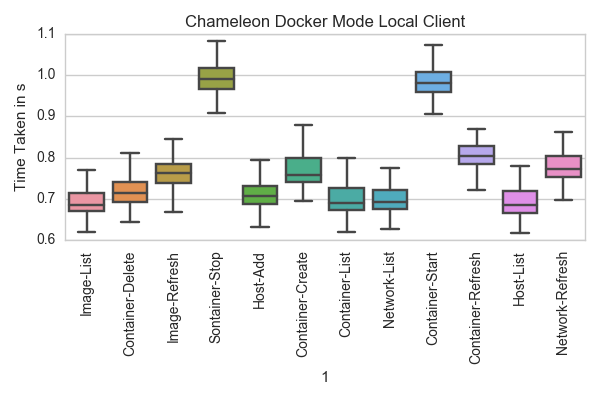
\includegraphics[width=0.8\linewidth]{images/Chameleon-Docker-Mode-Local-Client.png}}
\caption{Chameleon Docker Mode Local Client}
\label{fig:Chameleon-Docker-Mode-Local-Client}
\end{figure}


\begin{figure}[ht]
\centering
\fbox{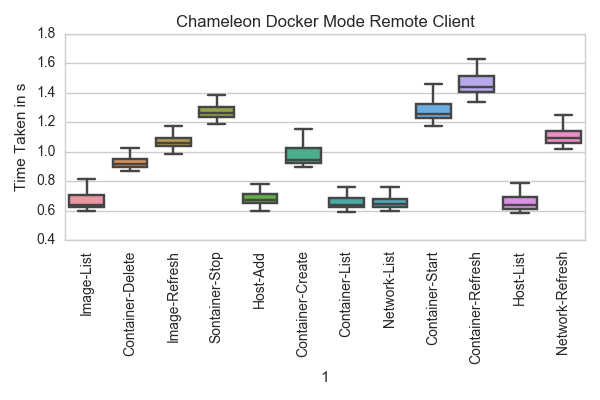
\includegraphics[width=0.8\linewidth]{images/Chameleon-Docker-Mode-Remote-Client.png}}
\caption{Chameleon Docker Mode Remote Client}
\label{fig:Chameleon-Docker-Mode-Remote-Client}
\end{figure}


\begin{figure}[h]
\centering
\fbox{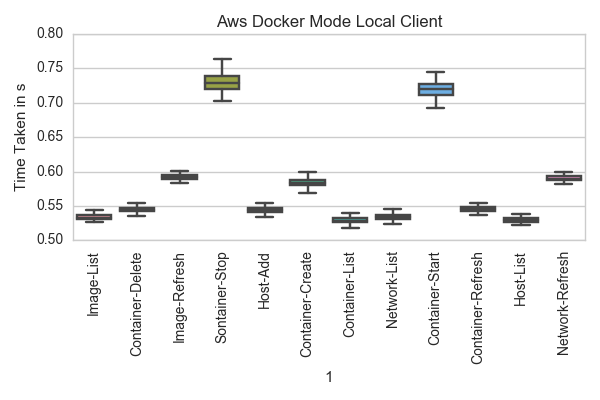
\includegraphics[width=0.8\linewidth]{images/Aws-Docker-Mode-Local-Client.png}}
\caption{Aws Docker Mode Local Client}
\label{fig:Aws-Docker-Mode-Local-Client}
\end{figure}


\begin{figure}[h]
\centering
\fbox{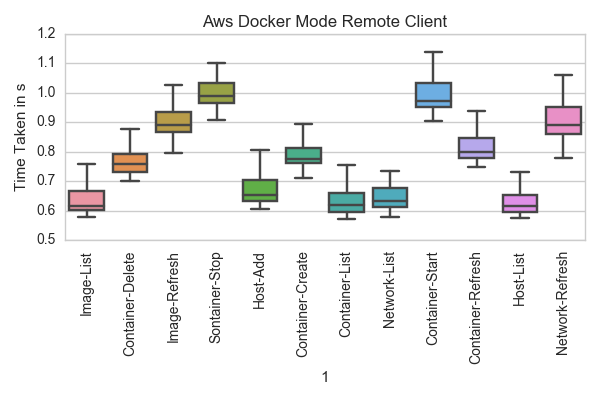
\includegraphics[width=0.8\linewidth]{images/Aws-Docker-Mode-Remote-Client.png}}
\caption{Aws Docker Mode Remote Client}
\label{fig:Aws-Docker-Mode-Remote-Client}
\end{figure}


Based on the benchmark reults we can infer the below details
\begin{enumerate}
\item  In the battle of the clouds Aws is around 20 percent faster than Chameleon cloud in docker mode
\item  Cloudmesh docker operations for the docker command performed in a local network are between
25 and 30  percent faster.We also noticed some network issues when performing the test from a
remote network however we chose to ignore those outliers in the plot.
\item The standard deviation of the response times is significantly lower for Aws than Chameleon indicating 
that Aws is much more stable and reliabe in performance than the chameleon cloud
\item The mean container create times range between 0.5 to 1 s which is significantly faster than normal VM 
boot times on the cloud .
\end{enumerate}

\begin{table}[h]
\centering
\caption{Docker Mode AWS VS Chameleon Local Vs Remote}
\label{Docker Mode AWS VS Chameleon Local Vs Remotel}
\begin{tabular}{|l|l|l|p{0.86cm}|l|p{0.86cm}|}
\hline
 & \textbf{} & \multicolumn{2}{c|}{\textbf{Aws}} & \multicolumn{2}{c|}{\textbf{Chameleon}} \\ \hline
 & \textbf{} & \textbf{Local} & \textbf{Remote} & \textbf{Local} & \textbf{Remote} \\ \hline
\textbf{Image-List} & mean & 0.534 & 0.661 & 0.695 & 0.704 \\
\textbf{Image-List} & std & 0.004 & 0.128 & 0.039 & 0.197 \\
\textbf{Container-Delete} & mean & 0.545 & 0.785 & 0.721 & 0.951 \\
\textbf{Container-Delete} & std & 0.004 & 0.090 & 0.040 & 0.115 \\
\textbf{Image-Refresh} & mean & 0.592 & 0.925 & 0.763 & 1.139 \\
\textbf{Image-Refresh} & std & 0.005 & 0.109 & 0.040 & 0.298 \\
\textbf{Sontainer-Stop} & mean & 0.730 & 1.017 & 0.992 & 1.299 \\
\textbf{Sontainer-Stop} & std & 0.014 & 0.122 & 0.041 & 0.113 \\
\textbf{Host-Add} & mean & 0.544 & 0.691 & 0.710 & 0.727 \\
\textbf{Host-Add} & std & 0.004 & 0.114 & 0.038 & 0.194 \\
\textbf{Container-Create} & mean & 0.584 & 0.798 & 0.767 & 1.007 \\
\textbf{Container-Create} & std & 0.006 & 0.075 & 0.042 & 0.164 \\
\textbf{Container-List} & mean & 0.529 & 0.655 & 0.697 & 0.689 \\
\textbf{Container-List} & std & 0.004 & 0.110 & 0.038 & 0.141 \\
\textbf{Network-List} & mean & 0.534 & 0.668 & 0.700 & 0.679 \\
\textbf{Network-List} & std & 0.005 & 0.098 & 0.035 & 0.115 \\
\textbf{Container-Start} & mean & 0.720 & 1.018 & 0.985 & 1.310 \\
\textbf{Container-Start} & std & 0.011 & 0.145 & 0.044 & 0.169 \\
\textbf{Container-Refresh} & mean & 0.546 & 0.824 & 0.805 & 1.509 \\
\textbf{Container-Refresh} & std & 0.004 & 0.070 & 0.033 & 0.208 \\
\textbf{Host-List} & mean & 0.530 & 0.659 & 0.693 & 0.708 \\
\textbf{Host-List} & std & 0.004 & 0.125 & 0.042 & 0.273 \\
\textbf{Network-Refresh} & mean & 0.591 & 0.946 & 0.780 & 1.137 \\
\textbf{Network-Refresh} & std & 0.005 & 0.171 & 0.043 & 0.151
\end{tabular}
\end{table}


\subsection{Swarm Mode - Results}

Below are the categories of the Benchmark results
\begin{enumerate}
\item Chameleon Swarm Mode Local Client Figure~\ref{fig:Chameleon-Swarm-Mode-Local-Client}
\item Chameleon Swarm Mode Remote Client Figure~\ref{fig:Chameleon-Swarm-Mode-Remote-Client}
\item Aws Swarm Mode Local Client Figure~\ref{fig:Aws-Swarm-Mode-Local-Client}
\item Aws Swarm Mode Remote Client Figure~\ref{fig:Aws-Swarm-Mode-Remote-Client}
\end{enumerate}

\begin{figure}[ht]
\centering
\fbox{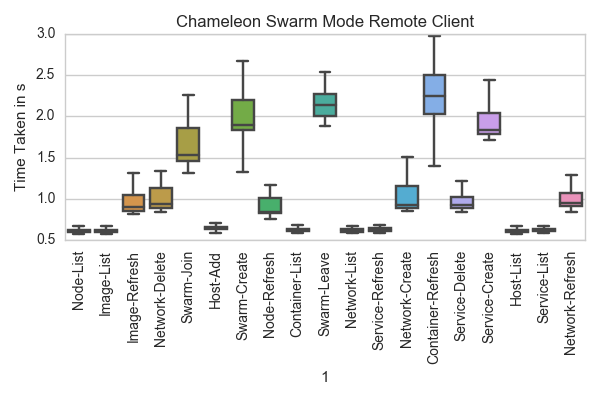
\includegraphics[width=0.8\linewidth]{images/Chameleon-Swarm-Mode-Remote-Client.png}}
\caption{Chameleon Swarm Mode Remote Client}
\label{fig:Chameleon-Swarm-Mode-Remote-Client}
\end{figure}

\begin{figure}[ht]
\centering
\fbox{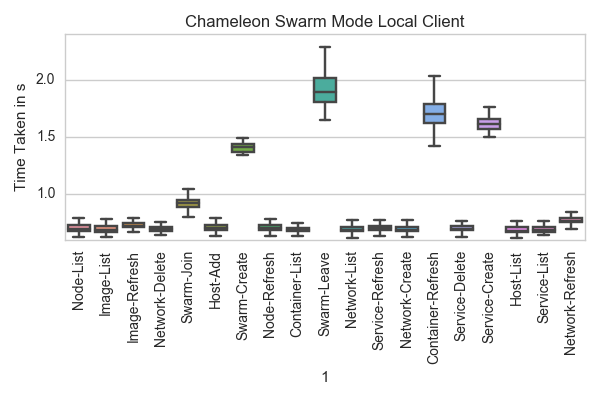
\includegraphics[width=0.8\linewidth]{images/Chameleon-Swarm-Mode-Local-Client.png}}
\caption{Chameleon Swarm Mode Local Client}
\label{fig:Chameleon-Swarm-Mode-Local-Client}
\end{figure}


\begin{figure}[h]
\centering
\fbox{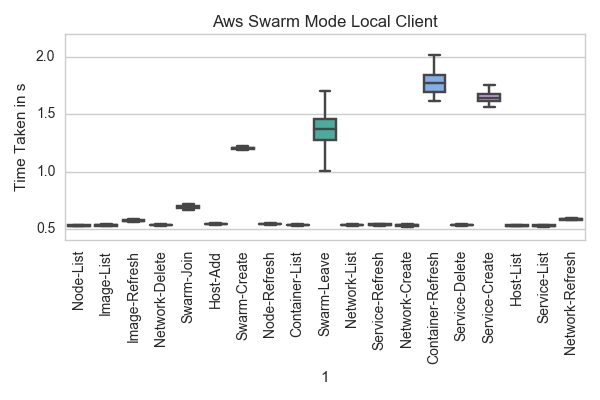
\includegraphics[width=0.8\linewidth]{images/Aws-Swarm-Mode-Local-Client.png}}
\caption{Aws Swarm Mode Local Client}
\label{fig:Aws-Swarm-Mode-Local-Client}
\end{figure}


\begin{figure}[h]
\centering
\fbox{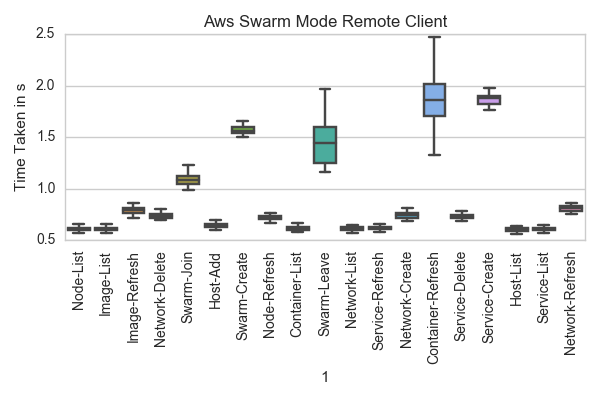
\includegraphics[width=0.8\linewidth]{images/Aws-Swarm-Mode-Remote-Client.png}}
\caption{Aws Swarm Mode Remote Client}
\label{fig:Aws-Swarm-Mode-Remote-Client}
\end{figure}

Based on the benchmark reults we can infer the below details
\begin{enumerate}
\item  In the battle of the clouds Aws is around 20 percent faster than Chameleon cloud in swarm mode
\item  Cloudmesh swarm operations for the swarm command performed in a local network are between
25 and 30  percent faster.
\item The standard deviation of the response times is significantly lower for Aws than Chameleon indicating 
that Aws is much more stable and reliabe in performance than the chameleon cloud
\item The mean service create times range between 2 to 1.6 s for 4 replicated containers 
which is significantly faster than normal boot times for a similar number of VM on the same  cloud .
\end{enumerate}

\begin{table}[h]
\centering
\caption{Swarm Mode AWS VS Chameleon Local Vs Remote}
\label{Swarm Mode AWS VS Chameleon Local Vs Remote}
\begin{tabular}{|l|l|l|p{.86cm}|l|p{0.86cm}|}
\hline
 &  & \multicolumn{2}{c|}{\textbf{Aws}} & \multicolumn{2}{l|}{\textbf{Chameleon}} \\ \hline
 &  & \textbf{Local} & \textbf{Remote} & \textbf{Local} & \textbf{Remote} \\ \hline
\textbf{Node-List} & mean & 0.529 & 0.612 & 0.704 & 0.631 \\
\textbf{Node-List} & std & 0.004 & 0.022 & 0.037 & 0.056 \\
\textbf{Image-List} & mean & 0.532 & 0.614 & 0.696 & 0.626 \\
\textbf{Image-List} & std & 0.004 & 0.041 & 0.039 & 0.053 \\
\textbf{Image-Refresh} & mean & 0.571 & 0.818 & 0.732 & 0.981 \\
\textbf{Image-Refresh} & std & 0.006 & 0.139 & 0.035 & 0.220 \\
\textbf{Network-Delete} & mean & 0.536 & 0.822 & 0.701 & 1.024 \\
\textbf{Network-Delete} & std & 0.005 & 0.280 & 0.035 & 0.247 \\
\textbf{Swarm-Join} & mean & 0.690 & 1.178 & 0.925 & 1.666 \\
\textbf{Swarm-Join} & std & 0.015 & 0.345 & 0.053 & 0.270 \\
\textbf{Host-Add} & mean & 0.542 & 0.653 & 0.714 & 0.665 \\
\textbf{Host-Add} & std & 0.005 & 0.062 & 0.035 & 0.076 \\
\textbf{Swarm-Create} & mean & 1.201 & 1.640 & 1.320 & 1.963 \\
\textbf{Swarm-Create} & std & 0.046 & 0.342 & 0.213 & 0.340 \\
\textbf{Node-Refresh} & mean & 0.542 & 0.738 & 0.714 & 0.911 \\
\textbf{Node-Refresh} & std & 0.004 & 0.107 & 0.039 & 0.127 \\
\textbf{Container-List} & mean & 0.533 & 0.622 & 0.696 & 0.638 \\
\textbf{Container-List} & std & 0.004 & 0.039 & 0.033 & 0.050 \\
\textbf{Swarm-Leave} & mean & 1.419 & 1.460 & 1.932 & 2.143 \\
\textbf{Swarm-Leave} & std & 0.275 & 0.288 & 0.241 & 0.186 \\
\textbf{Network-List} & mean & 0.532 & 0.625 & 0.698 & 0.625 \\
\textbf{Network-List} & std & 0.004 & 0.050 & 0.035 & 0.027 \\
\textbf{Service-Refresh} & mean & 0.536 & 0.631 & 0.710 & 0.645 \\
\textbf{Service-Refresh} & std & 0.004 & 0.089 & 0.039 & 0.099 \\
\textbf{Network-Create} & mean & 0.531 & 0.781 & 0.698 & 1.009 \\
\textbf{Network-Create} & std & 0.005 & 0.156 & 0.035 & 0.162 \\
\textbf{Container-Refresh} & mean & 1.666 & 1.846 & 1.693 & 2.273 \\
\textbf{Container-Refresh} & std & 0.374 & 0.348 & 0.181 & 0.386 \\
\textbf{Service-Delete} & mean & 0.535 & 0.781 & 0.704 & 0.991 \\
\textbf{Service-Delete} & std & 0.004 & 0.205 & 0.039 & 0.140 \\
\textbf{Service-Create} & mean & 1.661 & 1.905 & 1.636 & 1.938 \\
\textbf{Service-Create} & std & 0.071 & 0.164 & 0.115 & 0.273 \\
\textbf{Host-List} & mean & 0.529 & 0.608 & 0.693 & 0.629 \\
\textbf{Host-List} & std & 0.004 & 0.030 & 0.033 & 0.083 \\
\textbf{Service-List} & mean & 0.528 & 0.617 & 0.698 & 0.639 \\
\textbf{Service-List} & std & 0.005 & 0.052 & 0.035 & 0.075 \\
\textbf{Network-Refresh} & mean & 0.583 & 0.834 & 0.776 & 1.009 \\
\textbf{Network-Refresh} & std & 0.005 & 0.145 & 0.039 & 0.126
\end{tabular}
\end{table}

\clearpage
\section{Conclusion}

In this project we have succefully integrated docker and swarm capabilities into
cloudmesh client.We have also demonstrated its use for a practical use case of
setting up a Elastic search cluster in docker and swarm modes.We have also 
benchmarked the commands for multiple clouds(AWS and Chameleon) in both 
local and remote modes and detailed the results and insights.The ansible scripts
as part of the project along with the capabilities built in the cloudmesh docker 
application provide for a seamless capability in deploying and provisioning applications
in docker and swarm containers.


\section{Acknowledgement}

We acknowledge our professor Gregor von Laszewski and all associate instructors for helping us and guiding us throughout this project.

\section{Appendices}
Appendix A: Work Distribution
The co-authors of this report worked together on the design of the technical
solutions, implementation, testing and documentation. Below given is the work
 distribution
\begin{itemize}
\item Karthick Venkatesan
    \begin{itemize}
    \item Design and Implementation of Docker and Swarm Commands .
    \item Integration of Docker and Swarm Commands to Docker API.
    \item Integration to cloudmesh.common,cloudmesh.rest ,cloudmesh.cmd5 repositories.
    \item Framework definition and wrapper class built for Python-Eve
    \item Ansible scripts for docker image installation  and setup of etc hosts
    \item Test scripts for Docker and Swarm command
    \item Dockerfile for installation of cloudmesh.docker
    \item Create Benchmark scripts for Local and Remote Benchmarking on Chameleon and AWS
    \item Execute Benchmark scripts for Chameleon and Aws and plot the results in Ipython
    \item Scripts for setup of Elasticsearch docker cluster
    \item Benchmark Elastic search swarm  cluster using ESRally and dcoument reults
    \item Writing related sections in this report.
    \end{itemize}

\item Ashok Vuppuda
    \begin{itemize}
    \item Design of Docker and Swarm Commands .
    \item Integration into cloudmesh.rest
    \item Python EVE integration and implementation for docker and Swarm Modes
    \item Ansible scripts for docker installation
    \item Test application on Aws and Chameleon clouds
    \item Execute Benchmark scripts for Chameleon and Aws and plot the results in Ipython
    \item Benchmark Elastic search docker  cluster using ESRally and dcoument reults
    \item Writing related sections in this report.
    \end{itemize}
\end{itemize}


% Bibliography


\bibliography{references}
 


\newpage

\appendix


\end{document}
